\section {Важные с точки зрения влияния на ОС функции}
Здесь будут описаны в качестве примера механизмы удаления файла и создания процесса в Windows

\subparagraph {Удаление файлов}
Как мы можем видеть на рис.\ref{fig:filedelete}, у пользовательских программ есть 2 основных пути
для удаления файлов:
\begin {figure}[h]
	\centering
	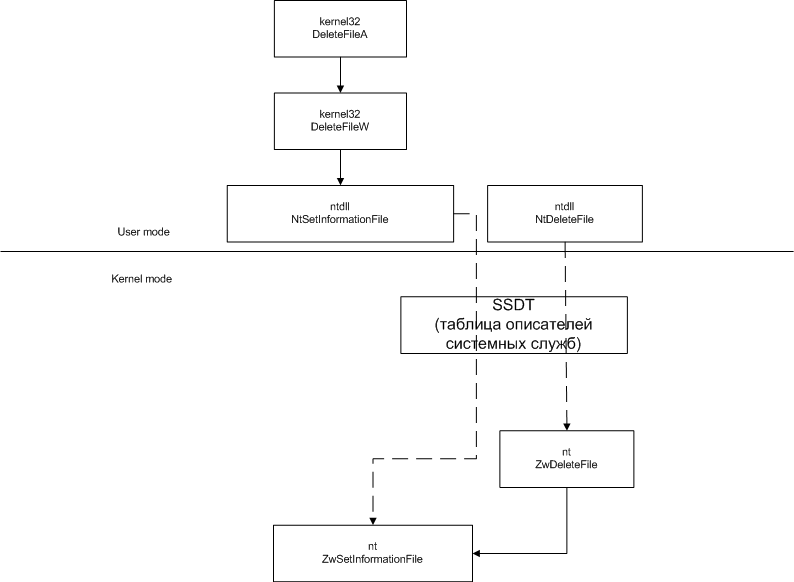
\includegraphics[width=\linewidth]{img/DeleteFileAPIs.png}
	\caption{Функции, отвечающие за удаление файлов}
	\label{fig:filedelete}
\end {figure}
\subparagraph {Создание процессов}
Для создания процессов есть множество различных путей, в том числе, и за рамками приводимых API функций, и нельзя полагаться, что любой создаваемый процесс будет обнаружен, если следить только за ними
\begin {figure}[h]
	\centering
	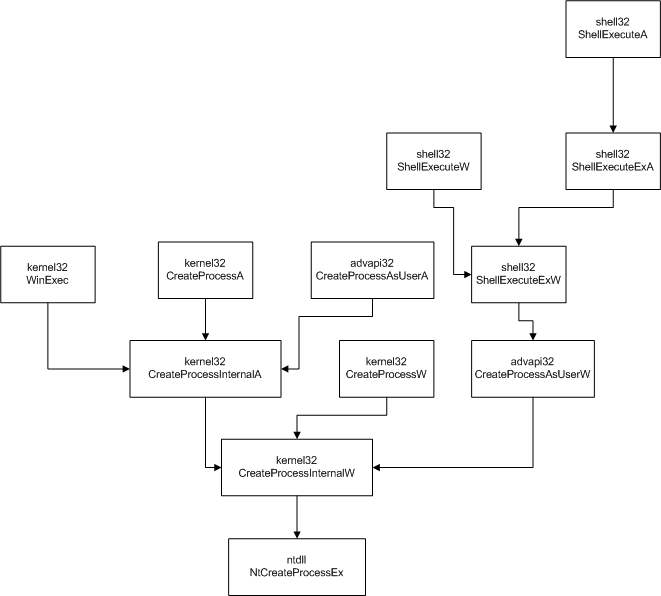
\includegraphics[width=\linewidth]{img/ExampleProcessCreateAPIs.png}
	\caption{Функции, отвечающие за создание процесса}
	\label{fig:createprocess}
\end {figure}